\documentclass{article}

\usepackage{amssymb, amsmath, amsthm, verbatim, graphicx}

\begin{document}


\renewcommand{\a}{\textbf{a}}
\renewcommand{\b}{\textbf{b}}
\renewcommand{\d}{\textbf{d}}
\newcommand{\e}{\textbf{e}}

\large

\begin{center}
\textbf{HW 11} \\  
MATH 611
\end{center}

\medskip


\medskip


\newcommand{\normal}{\mathcal{N}}

Reading
\begin{itemize}
\item Section $8.1$ introduces Bayesian networks.
\item Section $8.2$ discusses conditional independence.  
\end{itemize}


\begin{enumerate} 

\item The ASIA Bayesian network is a famous toy Bayesian network introduced in  \textit{Lauritzen and Spiegelhalter, Journal of the Royal Statistical Society, Series B, 1988}.   The article is attached.  See Figure 2 for the network and the start of section $4$ for a description of the node meanings.  The following website has a nice interface through which you can play with a fitted version of the model
\begin{verbatim}
https://www.bayesserver.com/examples/networks/asia
\end{verbatim}
The network has $8$ nodes. A sample $X \in \mathbb{R}^8$ from the network is decomposed as follows
\begin{align}
X &= (A, S, T, C, B, E, R, D) \\ \notag &= \text{(Asia, smoker, tuberculosis, cancer, bronchitis, either, x-ray, dyspnoea)}
\end{align}
Each $X_i \in \{0,1\}$, e.g. a person is either a smoker (0) or not (1).
\begin{enumerate}
\item Table $1$ in the paper provides the parameters to the model.  Show that given these parameters, $P(X)$ is completely determined for all $X$ in the sample space of $X$.
\item The paper presents the problem of computing $P(R=1 | A, S, D)$, with the intuition that knowledge of the probability of a positive X-ray will help a doctor determine if taking an x-ray is worthwhile.  Compute $P(R=1 | A=1, S=0, D=1)$  in two  ways,
\begin{enumerate}
\item Construct a Metropolis-Hastings sampler (or if you want to try, a Gibbs sampler) for $X$.  Use the sampler to estimate $P(R=1 | A=1, S=0, D=1)$.  (Use only $1$ run of your MH sampler and don't forget to allow a burn-in time).
\item Using the relation,
\begin{equation}
P(R=1 | A=1, S=0, D=1) = \frac{P(R=1, A=1, S=0, D=1)}{P(A=1, S=0, D=1)},
\end{equation}  
write down formulas for both the numerator and the denominator (these will be summations) and use R/Python to evaluate the formulas and, in turn, compute $P(R=1 | A=1, S=0, D=1)$.  (Note:  The small size of the network allows us to apply this explicit approach, but it would not be possible for a larger network) 
\end{enumerate}
\end{enumerate}

\item A third method we could implement to compute smoothing probabilities such as $P(R=1 | A=1, S=0, D=1)$ is a forward-backward iteration.  However, we have only considered this approach for a tree, and the $\delta$ (dsypnoea) and $\epsilon$ (either) nodes have two parents,  Instead, consider the tree shown below.   For the sake of time, we'll only consider writing down one step in these iterations, without actually implementing the iteration.    Assume that each node has as its states, $\{1,2,\dots,m\}$.
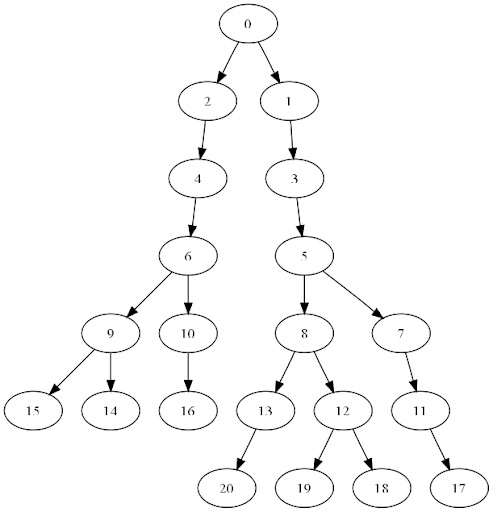
\includegraphics[width=0.9\textwidth]{tree.jpg}
\begin{enumerate}
\item Consider the backward iteration and suppose that we know $\beta_t(i)$ when the node $t$ is either node $9$ or node $10$.  Derive a formula for $\beta_t(i)$ for the case of $t$ equal to node $6$.  
\item Suppose we have completed the backward iteration and consider the forward iteration.  Suppose we know $\alpha_t(i)$ for $t$ as node $6$.  Derive a formula for $\alpha_t(i)$ for $t$ equal to node $9$.

\end{enumerate}
\end{enumerate}



\end{document}
